\documentclass{beamer}
\usepackage[utf8]{inputenc}
\usepackage{amssymb,amsmath,amsthm,mathtools}
\usepackage[english]{babel}

\usepackage{tikz}
\usetikzlibrary{calc} 
\beamertemplatenavigationsymbolsempty

\newcommand{\tr}{{\text{tr}}}
\newcommand{\B}[1]{\textbf{#1}}
\newcommand{\T}[1]{\texttt{#1}}

\title{A ququart SIC for ion trap quantum computers?}
\author{Matthew B. Weiss}
\institute{UMB: QBism Group}
\date{10/10/25}

\begin{document}

\frame{\titlepage}


\begin{frame}
\frametitle{Symmetric informationally complete sets}
\begin{center}
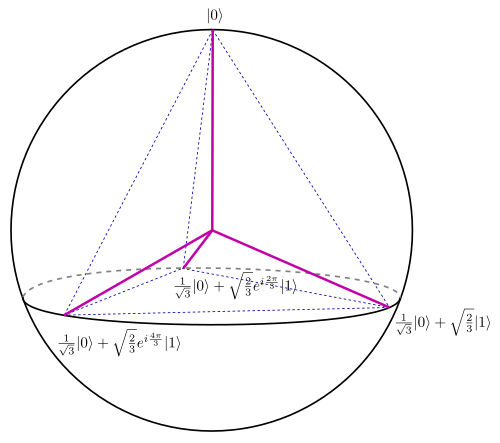
\includegraphics[scale=0.25]{img/qubit_sic}	
\end{center}
Fix a Hilbert space $\mathcal{H}_d$. If you can find a set of $d^2$ rank-1 projectors $\{\Pi_i\}$ satisfying
\begin{align}
	\tr(\Pi_{i}\Pi_{j})=\frac{d\delta_{i,j}+1}{d+1},
\end{align}
then you've found  regular simplex inscribed in quantum state-space: a SIC \cite{Renes_2004}!
\end{frame}

\begin{frame}
\frametitle{SIC's}
\begin{itemize}
\item SIC states (with a group covariance) have \emph{maximal magic} \cite{cuffaro2024quantumstatesmaximalmagic}.
\item The corresponding POVM $\{E_i = \frac{1}{d}\Pi_i\}$ is \emph{optimal for linear quantum state tomography} \cite{Scott2006}.
\item A SIC-based generalization of the double-split experiment demonstrates  the \emph{inherent contextuality} of quantum theory \cite{PhysRevLett.117.120404, heros}.
\item The numbers involved in constructing a SIC have \emph{deep algebraic number theoretic significance} \cite{Bengtsson_2017}. 
\item The question of whether SIC's exist in all dimensions directly relates to Hilbert's 12 problem about abelian extensions of the rationals \cite{appleby2025constructiveapproachzaunersconjecture}!
\end{itemize}
\end{frame}

\begin{frame}
\frametitle{Implementation}
\begin{center}
Is there a general method for implementing SIC-POVM's?
\vspace{1em}

First, let's consider its symmetries.	
\end{center}
	
\end{frame}


\begin{frame}
\frametitle{The Weyl-Heisenberg Group}
\begin{itemize}
\item 	Save one sporadic case, known SICs are ``WH-covariant.'' 
\item 
Fixing $\mathcal{H}_d$, let $\omega = e^{2\pi i /d}$ and define clock and shift operators,
\begin{align}
Z|m\rangle = \omega^{m}|m\rangle && 	X|m\rangle = |m+1\rangle && X=F^\dagger Z F,
\end{align}	
where $F$ is the DFT, as well as Weyl-Heisenberg displacement operators,
\begin{align}
D_{a,b} = X^a Z^b	.
\end{align}
\item The $d^2$ SIC states arise as the orbit of a ``fiducial'' state $\Pi$,
\begin{align}
	\Pi_{a,b}=D_{a,b} \Pi D_{a,b}^\dagger.
\end{align}
\end{itemize}
WH group covariance means:
\begin{itemize}
\item We can find fiducials more easily classically.
\item We can implement SICs more easily quantum mechanically.
\end{itemize}
\end{frame}

\begin{frame}
\frametitle{Historical flavor}
From \emph{Bell System Technical Journal}:
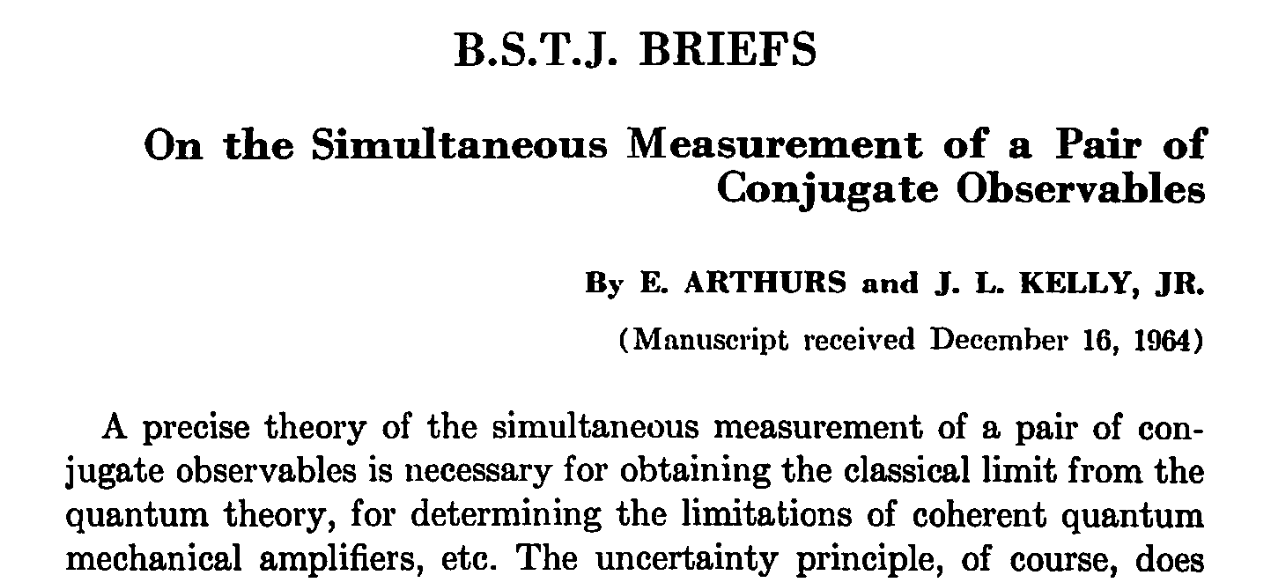
\includegraphics[scale=0.5]{img/ak_ref}	
\end{frame}

\begin{frame}
\frametitle{Arthurs-Kelly procedure}
\begin{itemize}
\item Prepare two ancillas in a special starting state.
\item Coherently shift ancilla 1 conditional on the position of the system.
\item Coherently shift ancilla 2 conditional on the momentum of the system.
\item Measure the ancillas.
\end{itemize}
 Realizes a ``Weyl-Heisenberg covariant POVM'' on the system.

\begin{itemize}
\item E.g., a coherent state measurement, or ``heterodyne'' measurement in optics.
\item Can be adapted to qudits: in particular, for a SIC measurement.
\end{itemize}
	
\end{frame}




\begin{frame}
\frametitle{Qudit Arthurs-Kelly}
\begin{itemize}
	\item Let $\{|k \rangle\}$ denote discrete position states (the computational basis).
\item Let  $\{|m\rangle_p=F|m\rangle\}$ denote discrete momentum states.
\item The Arthurs-Kelly unitary is:
\begin{align}
U_{AK} &= \left(\sum_m I \otimes X^{-m} \otimes |m\rangle_p\langle m|_p	\right)\left(\sum_k X^{-k} \otimes I \otimes |k\rangle\langle k|\right).
\end{align}
\item But how to  prepare the ancillas given the desired fiducial state?
\end{itemize}

\end{frame}

\begin{frame}
\frametitle{Qudit Arthurs-Kelly}
\begin{itemize}
 \item To prepare the ``ready state'' of the two ancillas,
\begin{align}
U_{PA} &= 	\left(\sum_j |j\rangle\langle j|\otimes Z^j	\otimes I\right)\Big(I \otimes F^\dagger \otimes I\Big).
\end{align}
\item Let $|\phi\rangle$ be a SIC fiducial, and $|\psi\rangle$  the system state, then
\begin{align}
|\text{post-interaction}\rangle=U_{AK}U_{PA}\Big(|\phi^*\rangle	\otimes |\phi\rangle \otimes |\psi\rangle\Big).
\end{align}
\item 	Measuring the two ancillas gives $d^2$ possible outcomes with \begin{align}
 	P(a,b)=\frac{1}{d}\tr(\Pi_{a,b}\rho).
 \end{align}
\item Afterwards, the system is projected into the SIC state $\Pi_{a,b}$.
\end{itemize}
\end{frame}

\begin{frame}
	\begin{center}
	But actually, there's a simpler way.	
	\end{center}

\end{frame}

\begin{frame}
	\frametitle{Thrifty SIC}
\begin{itemize}
\item Let  $|\psi\rangle$ an arbitrary state, and $|\phi\rangle$ be the fiducial.
\begin{align}
&\Big(\langle a| \otimes \langle b|\Big)(I\otimes F^\dagger)\left(\sum_j X^{-j}\otimes |j\rangle\langle j|\right)\Big(|\psi\rangle \otimes |\phi^*\rangle	\Big)\nonumber\\
&=\frac{1}{\sqrt{d}}\langle \phi |D_{a,b}^\dagger |\psi\rangle.
\end{align}
\item The probabilities for a computational basis measurement are precisely the SIC probabilities.
\item  Just one ancilla!
\item  But afterwards, the state is projected into a computational basis state.
\end{itemize}
\end{frame}

\begin{frame}
\frametitle{Trade-offs}
\begin{itemize}
\item The Arthurs-Kelly implementation requires two ancillas, and consequently a more involved interaction.
\item The ``thrifty'' implementation requires just one ancilla. 
\item The downside is that the system is not projected into a SIC state afterwards: relevant when you are measuring a subsystem of a multipartite system.
\item The upside is you can do cheaper tomography!
\end{itemize}
	
\end{frame}



\begin{frame}
\frametitle{Why we care about a $d=4$ SIC}
\begin{center}
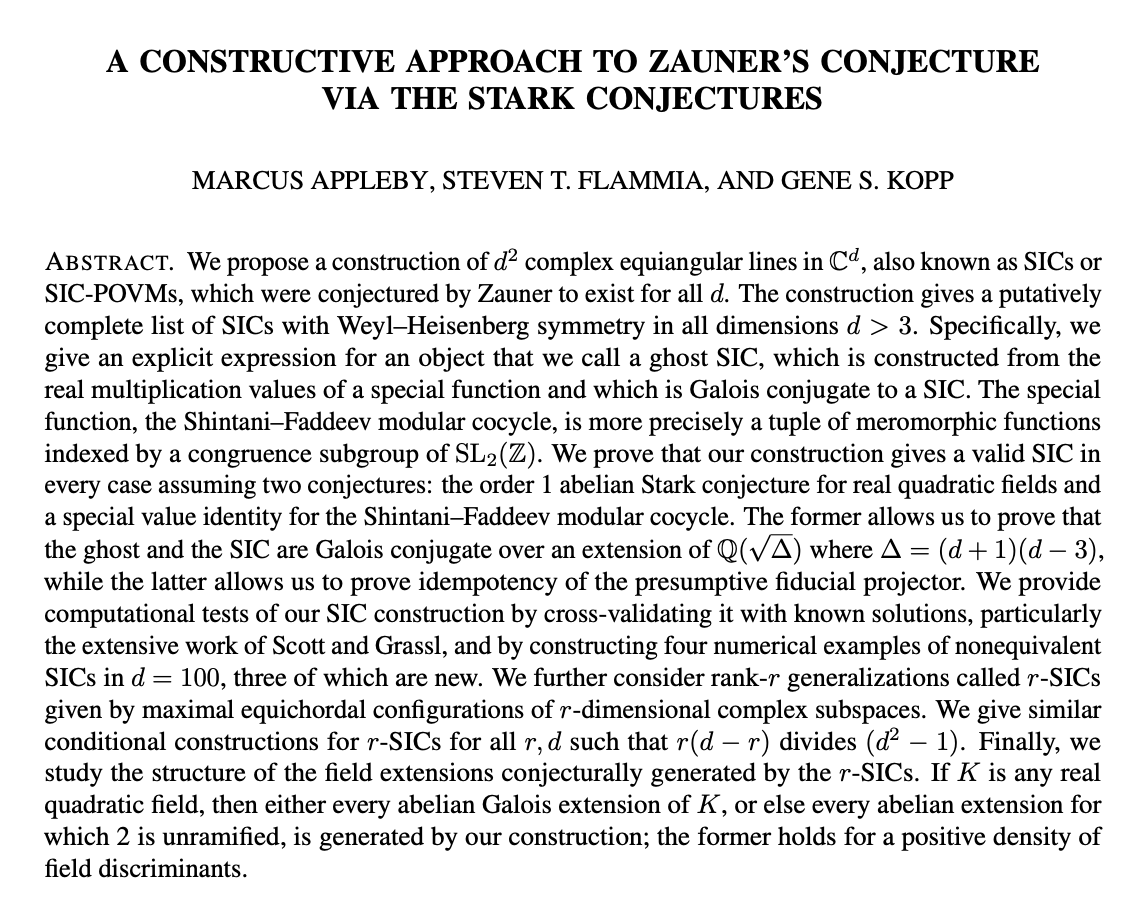
\includegraphics[scale=0.4]{img/number_theory}	
\end{center}
\end{frame}

\begin{frame}
\frametitle{Why we care about a $d=4$ SIC}
\begin{itemize}
\item $d=4$ is the first dimension for which the amplitudes defining a SIC have a distinctive number theoretic character.
\item The number theory provides a systematic framework for constructing SICs: a tantalizing intersection of pure math and physics whose ramifications have yet to be fully explored.
\item Also, of course, $d=4$ is the first dimension you can compare two qubit tomography to ququart tomography. Qubits are not the future! 
\item Finally, we want to do SICs not because they are easy, but because they are hard! To stretch the technology, provide a stress test for quantum hardware.  
\end{itemize}	
\end{frame}



\begin{frame}
\frametitle{A $d=4$ fiducial}
Exploit the ``monomial representation'' \cite{monomial} to write
\begin{align}
\label{fiducial}
&|\phi\rangle = \nonumber\\
&	(H \otimes I)\begin{pmatrix}1 & 0 & 0 & 0\\ 0 & e^{i\pi(-1/4)} & 0 & 0 \\ 0 & 0 & e^{i\pi (1/4)} & 0 \\ 0 & 0 & 0 & e^{i\pi (1/2)}\end{pmatrix}\frac{1}{\sqrt{5+\sqrt{5}}}\begin{pmatrix} \sqrt{2+\sqrt{5}} \\ 1 \\ 1 \\ 1 \end{pmatrix},
\end{align}	
where $H$ is the qubit Hadamard gate. 	
\end{frame}

\begin{frame}
\frametitle{A $d=4$ fiducial}
As a circuit on two qubits:
\begin{center}
 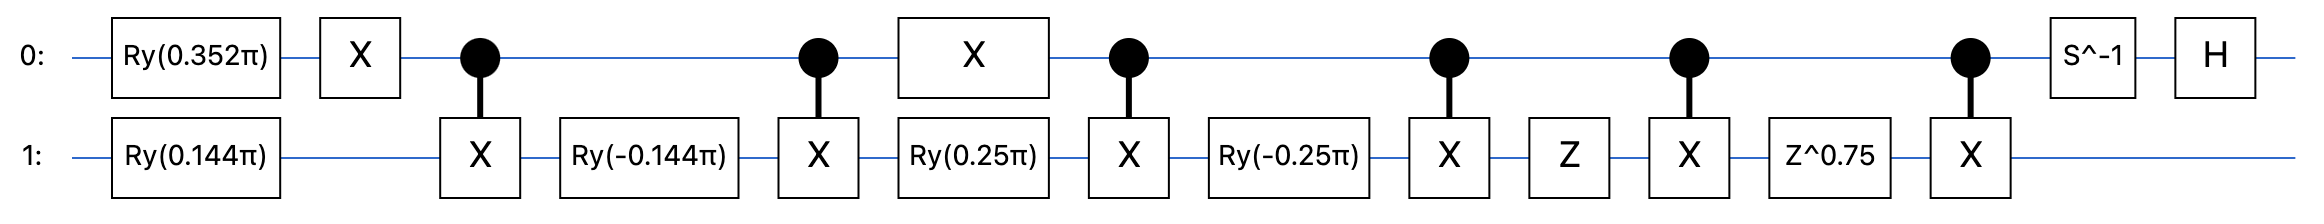
\includegraphics[scale=0.28]{img/fiducial_prep}
\end{center}   
   \end{frame}


\begin{frame}
\frametitle{Ion traps}
\begin{itemize}
\item In ``Experimental single-setting quantum state tomography'', you implement a qubit SIC using a native quqart \emph{locally}.
\item Can we similarly realize a ququart SIC using a sixteen level ion? Or with two (or three) native ququarts? 
\item In ``A universal qudit quantum processor with trapped ions,'' you implement $d=7$ qudits, and show in general how to implement a controlled exchange gate $C_{\text{EX}}$ from which one can implement $C_{\text{SUM}}$, that is, the controlled shift $CX$.
\item If doing $CX, CZ$, and $F$ are easy, then the only difficulty is in preparing the fiducial itself!
\end{itemize}
	
\end{frame}




\begin{frame}
\frametitle{Take 3: A block-diagonal scheme}
\begin{itemize}
	\item Both of the methods presented so far separate out the preparation of the fiducial from the implementation of the measurement itself.
	\item Exploiting WH symmetry, one may more directly construct a unitary  which implements a SIC: even better, the unitary can be block-diagonalized in a straightforward way.
	\item In particular, the method can be tailored to the monomial representation of the $d=4$ fiducial.
	\item (Originally developed for a quantum optics set-up.)
\end{itemize}		
\end{frame}

\begin{frame}
\frametitle{Take 3: A block-diagonal scheme}
Let $\lambda = e^{i\pi /4}$, and define gates
\begin{align*}
        D &= \frac{1}{\sqrt{2}}
            \begin{pmatrix}
                1 & 1\\
                i & -i
            \end{pmatrix} ,
        L_\pm = \frac{1}{\sqrt{2}}
            \begin{pmatrix}
            \mp \lambda & 1 \\
             \pm \lambda & 1
            \end{pmatrix}
        \\
        R_1 &= \frac{1}{\sqrt{2}\lambda}
            \begin{pmatrix}
            1 & -1 \\
             \lambda & \lambda
            \end{pmatrix},
            \
        R_2 = \frac{1}{\sqrt{2}\lambda}
            \begin{pmatrix}
            \lambda & \lambda \\
            1 & -1
            \end{pmatrix},
\end{align*}
\begin{align*}
    U_{0/1} = \frac{1}{\sqrt{2}}
    \begin{pmatrix}
     u \pm i \lambda  & -1 \pm i \lambda  &  -i u \mp \lambda & i \mp \lambda \\
    -1 \mp i \lambda & -u \pm i \lambda  & i \pm \lambda & iu \mp \lambda\\
    -1 \pm i \lambda  u & -1 \mp i \lambda  & i \mp \lambda  u & i \pm \lambda \\
    -1 \pm i \lambda  & 1 \pm i \lambda  u & i \mp \lambda & -i \mp \lambda u\\
    \end{pmatrix}
\end{align*}

\begin{align*}
    U_{2/3} = \frac{1}{\sqrt{2}}
    \begin{pmatrix}
    1 \pm \lambda & i (1 \pm \lambda  u) & i (1 \mp \lambda) & -1 \pm \lambda  u \\
   1 \pm \lambda  u & -i (1 \pm \lambda) & i (1 \mp \lambda u) & 1 \mp \lambda  \\
    -1 \pm \lambda & i (u \mp \lambda ) & -i (1 \pm \lambda ) & -u \mp \lambda \\
    u \mp \lambda  & i (1 \mp \lambda) & i (u \pm \lambda ) & -1 \mp 
    \lambda
    \end{pmatrix}
\end{align*}
\end{frame}

\begin{frame}
\frametitle{Take 3: A block-diagonal scheme}
\begin{small}
Suppose the ion has 16 energy levels, and the state to be measured is prepared as a superposition of every 4th level $(a, b, c, d)$. 
\end{small}
\begin{center}
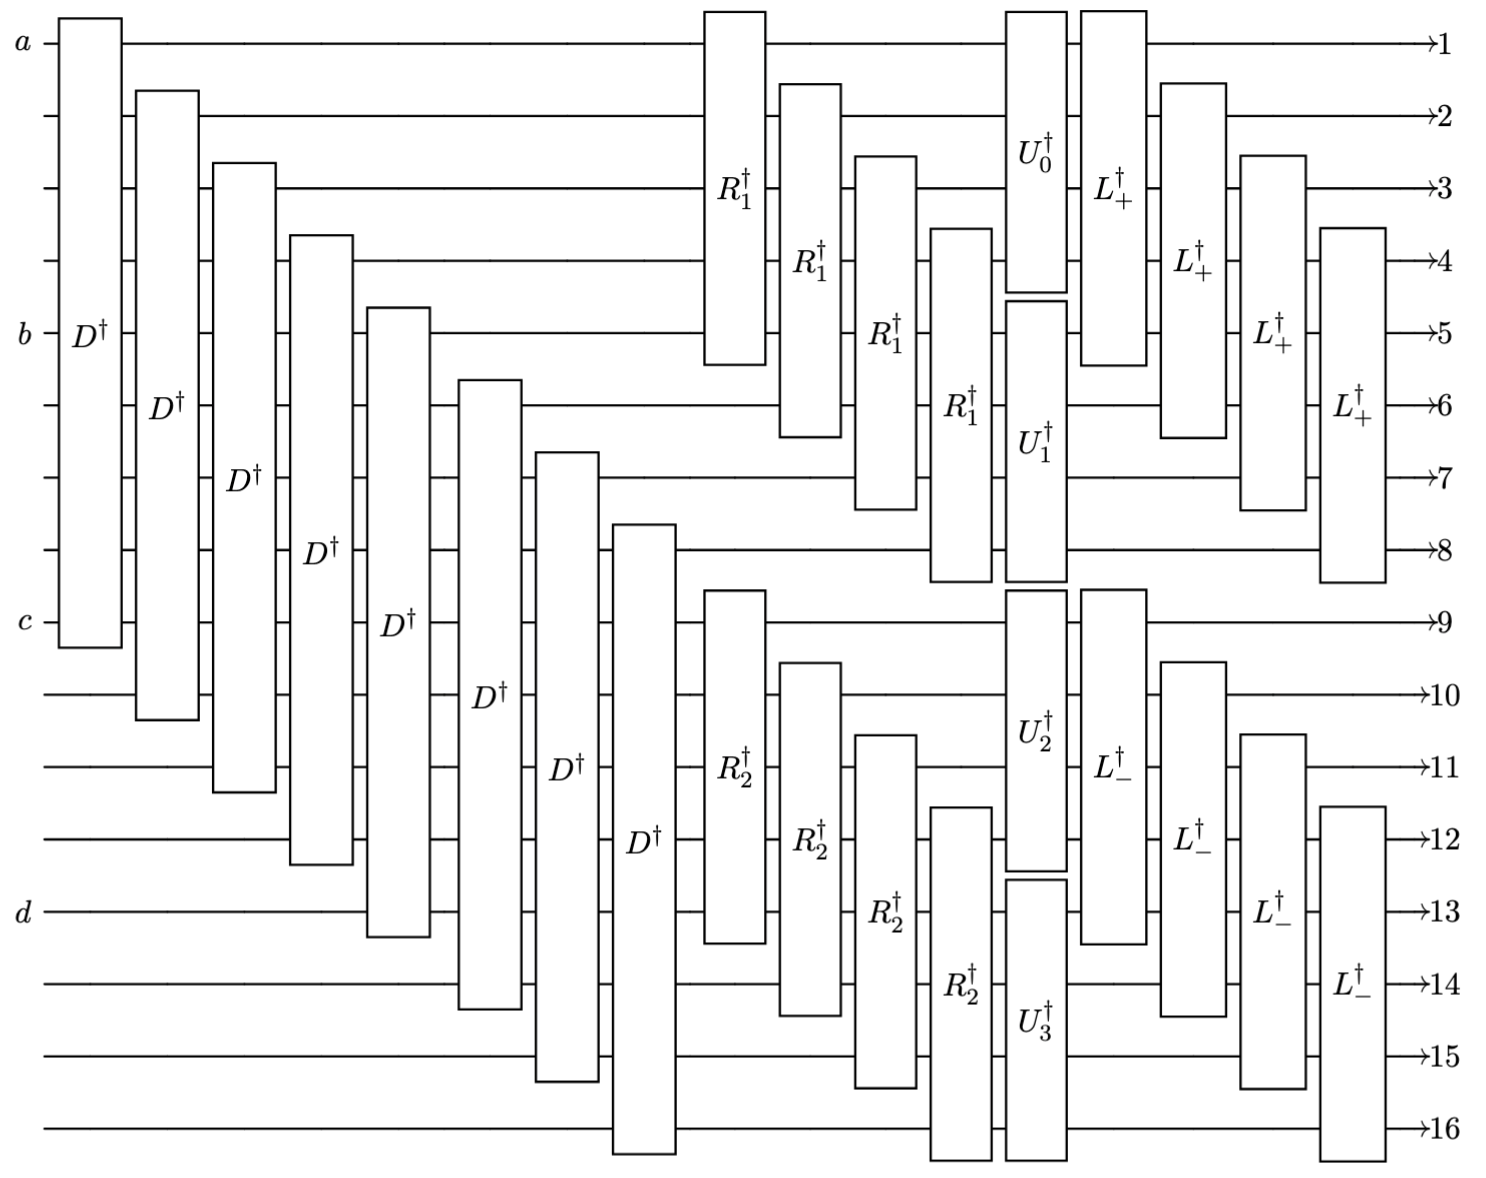
\includegraphics[scale=0.3]{img/sachin16}	
\end{center}
\begin{small}
Here $U_0, U_1, U_2, U_3$ act on four degrees of freedom. The other gates act only the first and last degrees of freedom encompassed by the gate.
\end{small}
\end{frame}

\begin{frame}
\begin{center}
Now we know how to perform SIC's. 
\vspace{2em}

But what can we do with them?
\end{center}
	
\end{frame}


\begin{frame}
\frametitle{From tomography to the Born rule}
\begin{itemize}
\item Reconstructing density matrices from SIC probabilities:
\begin{align}
\rho = \sum_i \left[(d+1)P(R_i)- \frac{1}{d}\right]\Pi_i	,
\end{align}
where $P(R_i)=\frac{1}{d}\tr(\Pi_i\rho)$.
\item Leads to an elegant reformulation of the Born rule as a consistency rule for probability assignments.
\item Checking that probability assignments are consistent according to this rule  provides a way to validate quantum hardware!
\end{itemize}
\end{frame}


\begin{frame}
\frametitle{The Born Rule}
\vspace{-2em}
\begin{center}
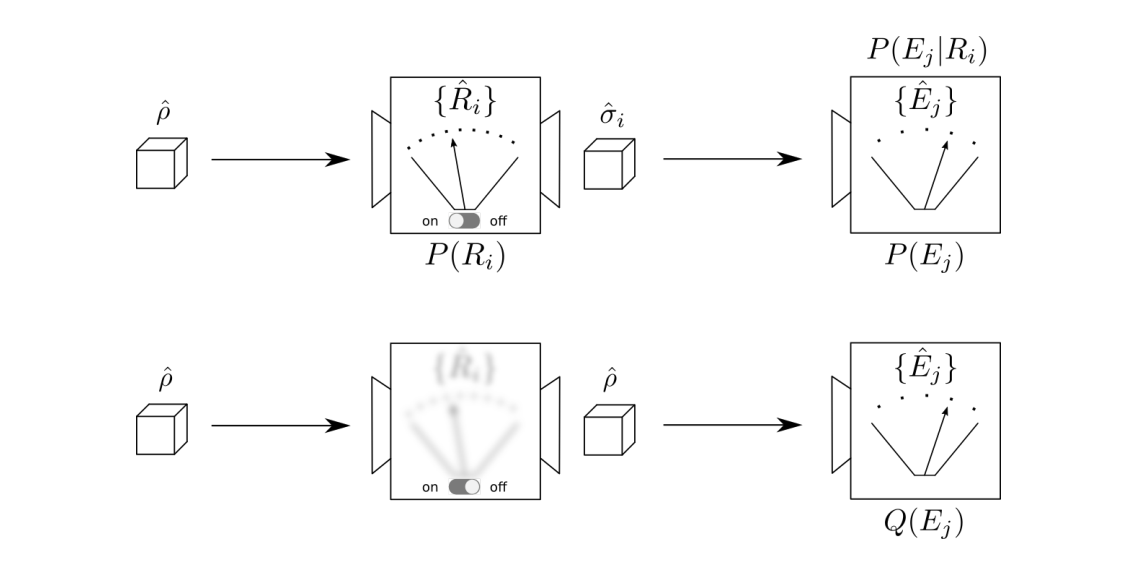
\includegraphics[scale=0.45]{img/sky_ground}	
\end{center}
\vspace{-2em}
\begin{small}
\begin{align}
P(E_j) &= \sum_i P(E_j|R_i)P(R_i)\\
Q(E_j) &= \sum_{ik} P(E_j|R_i)\Phi_{ik}P(R_k)
\end{align}
where $\Phi = P(R|R)^{-1}$ for any linearly independent $\{R_i\}$ and $\{\sigma_i\}$.\end{small}
\end{frame}

\begin{frame}
\frametitle{The Born Rule}
\begin{itemize}
\item In particular, for a SIC:
\begin{align}
Q(E_j) &=\sum_{i} P(E_j|R_i)\left[(d+1)P(R_i)-\frac{1}{d}\right]	.
\end{align}	
\item Among all IC-POVMs with $d^2$ elements, $\lVert I - \Phi \rVert$ achieves its minimum only for SIC's.
\item Other measurements artificially exaggerate the difference between classical and quantum! In this way, the SICs provide a good standard measurement.
\item  Let $W(E_j)=(d+1)P(R_i)-\frac{1}{d}$: these are quasiprobabilities. 
\item Their negativity diagnoses contextuality.
\item The more noise, the less negativity.
\end{itemize}
	
\end{frame}

\begin{frame}
\frametitle{Consistency}
Let us consider the following concrete set of experiments:
\begin{enumerate}
\item Prepare the SIC states in turn, and then a SIC measurement. Yields matrix of probabilities $P_{ij}=P(R_i|R_j)$.
\item Prepare the computational basis states $\{\Pi_i=|i\rangle\langle i|\}$, and then performing a SIC. Yields probabilities $p_{ij} = P(R_j|\Pi_i)$.
\item Prepare the SIC states, and a computational basis measurement: $C_{ij}=P(\Pi_i|R_j)$.
\item Prepare the computational basis states, and then a computational basis measurement: $q_{ij}=P(\Pi_i|\Pi_j)$.
\end{enumerate}
	Letting $\Phi=P^{-1}$, the Born rule then demands the following consistency criterion,
\begin{align}
q = C\Phi p.	
\end{align}
How well can we approximate this in the presence of noise? To what extent can we minimize $ \lVert q - C\Phi p	\rVert$?
\end{frame}

\begin{frame}
\frametitle{Metrics of success}
\begin{itemize}
	\item $\lVert P_{\text{SIC}}-P	\rVert$
	\item $ \lVert \Phi_{\text{SIC}}-\Phi	\rVert$
	\item $\lVert I - \Phi	\rVert$
	\item $\lVert q - C\Phi p	\rVert$
	\item Average negativity of quasiprobabilities over random states.
	\item Further, compare performance against other WH-POVM's with less magic (that is, for alternative choices of fiducials).
	\item If enough precision is available, could we use variational algorithms to \emph{learn} SIC fiducials themselves by tuning ansatz parameters?
\end{itemize}	
\end{frame}



\begin{frame}[allowframebreaks]
\frametitle{Bibliography}
\bibliographystyle{plain} 
\bibliography{QuditArthursKelly}
\end{frame}

\end{document}
